\chapter{Introduction}
\label{chap:introduction}

% This is the introduction where you should introduce your work. In
% general the thing to aim for here is to describe a little bit of the
% context for your work -- why did you do it (motivation), what was the
% hoped-for outcome (aims) -- as well as trying to give a brief overview
% of what you actually did.
%
% It's often useful to bring forward some ``highlights'' into this
% chapter (e.g.\ some particularly compelling results, or a particularly
% interesting finding).
%
% It's also traditional to give an outline of the rest of the document,
% although without care this can appear formulaic and tedious. Your
% call.


\section{Context}
\label{sec:context}
% "describe a little bit of the context for your work"

\section{Motivation}
\label{sec:motivation}
% "why did you do it (motivation)"


\begin{figure}[H]
    \centering
    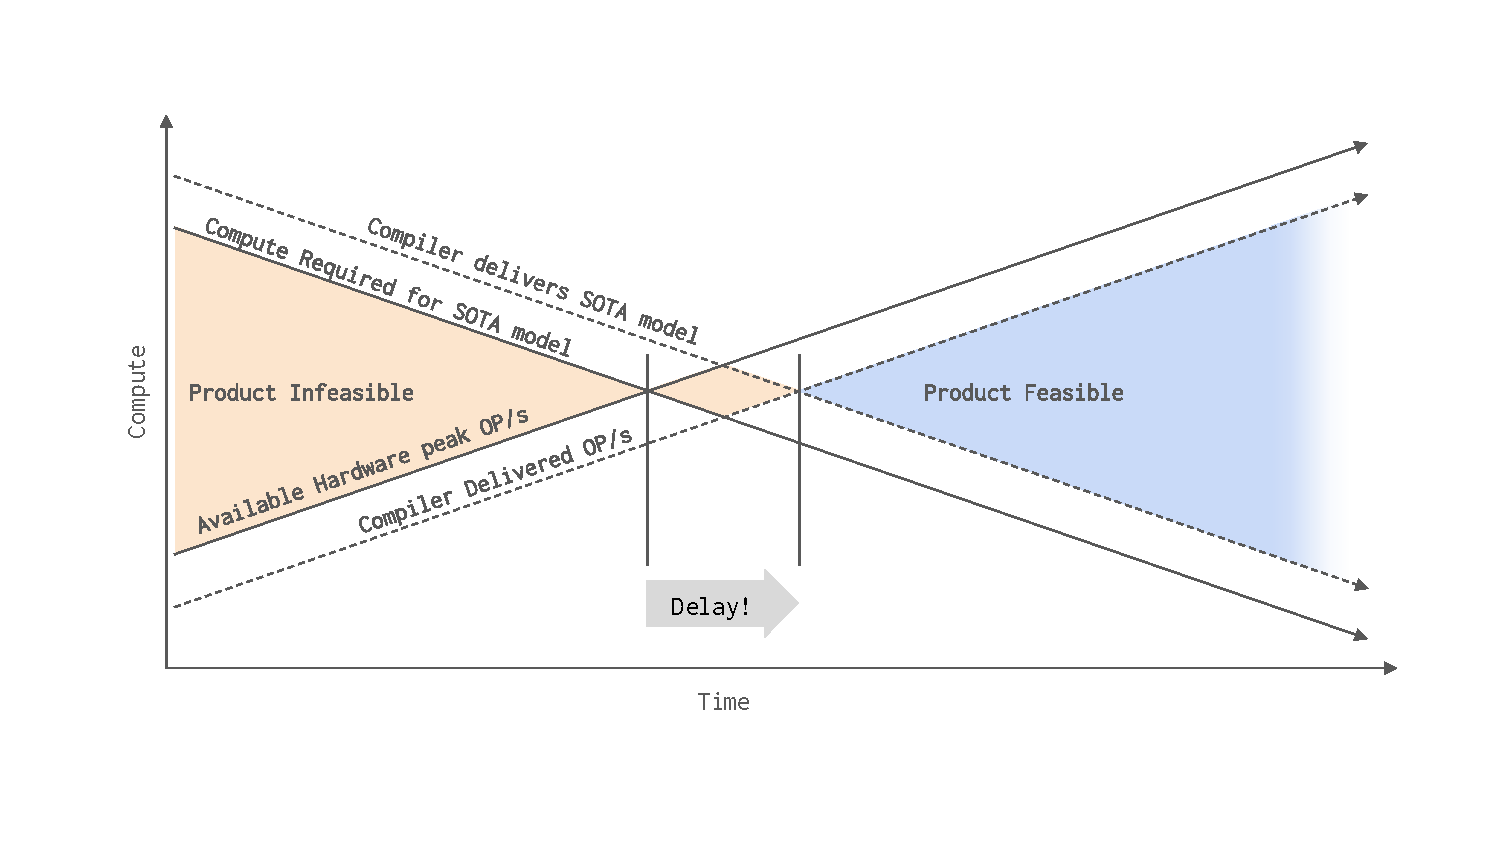
\includegraphics[width=\textwidth]{images/11_introduction/compilers_lagging.pdf}
    \caption{Compilers are lagging behind the development of both machine learning hardware and workloads. Figure created by Anton Lydike based on a slide from Sean Silva's talk at the March 2025 Cambridge Compiler Social.}
    \label{fig:compilers-lagging}
\end{figure}

\section{Aims}
\label{sec:aims}
% "what was the hoped-for outcome (aims)"

\section{Contributions}
\label{sec:contributions}
% "give a brief overview of what you actually did"


The contributions of our work are as follows:

\textbf{xDSL benchmarks and benchmarking infrastructure.}

\textbf{Comparison of xDSL and MLIR performance.}

\textbf{Analysis of the suitability of dynamic languages for dynamic workloads.}

\textbf{Optimisation of specialised xDSL pattern rewriter.}

% In this work we make the following contributions:

% \begin{enumerate}
%     \item The development of benchmarks and benchmarking infrastructure for the xDSL compiler framework
%     \item A comparison of the performance of MLIR and xDSL, disentangling the contributions of their language runtimes and implementation details
%     \item A discussion of the suitability of dynamic languages for dynamic workloads, such 
%     \item 
% \end{enumerate}